\begin{enumerate}
    \item Để tiện tính toán, ta đánh số các nam châm như hình dưới đây. \\
    \begin{figure}[!ht]
        \centering
        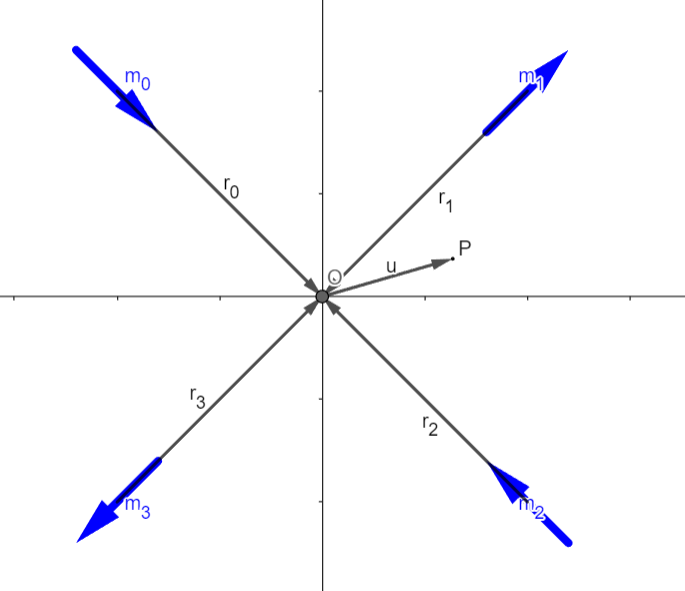
\includegraphics[scale = .5]{Problem_18/quadrupole.png}
      %  \caption{Caption}
    \end{figure}
    Từ trường tại điểm P có tọa độ $\Vec{r} = x\hat{x}+y\hat{y}$ là:
    \begin{equation} \label{eq1_Strong_Focusing}
        \Vec{B}= \sum_{i=0}^{3} \frac{\mu_0}{4\pi r_i'^5}\left[3(\Vec{m}_i\cdot \Vec{r'}_i)\Vec{r'}_i-\Vec{m}_i r_i'^2\right].
    \end{equation}
    Với $\Vec{r'}_i= \Vec{r}_i+\Vec{r}, \quad |\Vec{r}|/a \ll 1$, từ đây ta có
    \begin{equation} \label{eq2_Strong_Focusing}
        \frac{1}{r_i'^3}\approx\frac{1}{a^3}\left(1-\frac{3\Vec{r}_i \cdot \Vec{r}}{a^2}\right), \quad  \frac{1}{r_i'^5}\approx\frac{1}{a^5}\left(1-\frac{5\Vec{r}_i\cdot \Vec{r}}{a^2}\right).
    \end{equation}
        Thế (\ref{eq2_Strong_Focusing}) vào phương trình (\ref{eq1_Strong_Focusing}) ta thu được
    \begin{equation} \label{eq3_Strong_Focusing}
            \Vec{B} = \sum_{i=0}^{3} \frac{\mu_0}{4\pi}\left[\frac{3(\Vec{m}_i\cdot \Vec{r'}_i)\Vec{r'}_i}{a^5}\left(1-\frac{5\Vec{r}_i \cdot \Vec{r}}{a^2}\right)-\frac{\Vec{m}_i}{a^3}\left(1-\frac{3\Vec{r}_i \cdot \Vec{r}}{a^2}\right)\right].
    \end{equation}
    Ta lần lượt tính các số hạng thành phần của từ trường:
    \begin{equation} \label{eq4_Strong_Focusing}
        \Vec{m}_i\cdot \Vec{r}_i= (-1)^ip_m \cdot a\Longrightarrow \sum_{i=0}^{3}\Vec{m}_i \cdot \Vec{r'}_i= \sum_{i=0}^{3}\Vec{m}_i \cdot \Vec{r}+\sum_{i=0}^{3}(-1)^ip_m \cdot a=0,
    \end{equation}
    và
    \begin{equation} \label{eq5_Strong_Focusing}
    \begin{split}
        \sum_{i=0}^{3}(\Vec{m}_i \cdot \Vec{r'}_i)\Vec{r'}_i &=\sum_{i=0}^{3}(\Vec{m}_i \cdot \Vec{r}_i)\Vec{r}_i+\sum_{i=0}^{3}(\Vec{m}_i \cdot \Vec{r})\Vec{r}_i+\sum_{i=0}^{3}(\Vec{m}_i \cdot \Vec{r'}_i)\Vec{r}\\
        &=p_ma\sum_{i=0}^{3}(-1)^i\Vec{r}_i+\sum_{i=0}^{3}(\Vec{m}_i \cdot \Vec{r})\Vec{r}_i \\
        &=\sum_{i=0}^{3}(\Vec{m}_i\cdot \Vec{r})\Vec{r}_i= \sum_{i=0}^{3}\left[\Vec{r}\times (\Vec{r}_i \times\Vec{m}_i)+\Vec{m}_i(\Vec{r}_i \cdot\Vec{r})\right]\\
        &=\sum_{i=0}^{3}\Vec{m_i}(\Vec{r}_i \cdot\Vec{r}).
    \end{split}
    \end{equation}
    Thế (\ref{eq4_Strong_Focusing}) và (\ref{eq5_Strong_Focusing}) vào (\ref{eq3_Strong_Focusing}) và giữ lấy hệ thức bậc nhất theo $\Vec{r}$, ta thu được:
    \begin{equation} \label{eq6_Strong_Focusing}
        \begin{split}
            \Vec{B}&= \sum_{i=0}^{3} \frac{\mu_0}{4\pi}\left[\frac{6(\Vec{r}_i \cdot \Vec{r})\Vec{m}_i}{a^5}-\frac{15(\Vec{m}_i \cdot \Vec{r}_i )(\Vec{r}_i \cdot \Vec{r})\Vec{r}_i}{a^7}\right]\\
            &=\sum_{i=0}^{3} \frac{\mu_0}{4\pi}\left[\frac{6(\Vec{r}_i\cdot \Vec{r})\Vec{r}_i(-1)^ip_m}{a^6}-\frac{15(-1)^ip_m(\Vec{r}_i \cdot \Vec{r})\Vec{r}_i}{a^6}\right]\\
            &=-\sum_{i=0}^{3} \frac{\mu_0}{4\pi}\frac{9(\Vec{r}_i\cdot \Vec{r})\Vec{r}_i (-1)^ip_m}{a^6}\\
            &=- \frac{\mu_0}{4\pi}\frac{18p_m}{a^6}\left[(\Vec{r}_0 \cdot \Vec{r})\Vec{r}_0-(\Vec{r}_1\cdot \Vec{r})\Vec{r}_1 \right].
        \end{split}
    \end{equation} 
    Thay $\Vec{r}_0 = \frac{a}{\sqrt{2}}(\hat{x}-\hat{y})$ và $\Vec{r}_1= \frac{a}{\sqrt{2}}(\hat{x}+\hat{y})$, ta tìm được biểu thức từ trường
    \begin{equation} \label{eq7_Strong_Focusing}
        \Vec{B}=- \frac{\mu_0}{4\pi}\frac{9p_m}{a^4}\left[(x-y)(\Vec{x}-\Vec{y})-(x+y)(\Vec{x}+\Vec{y})\right]= \frac{9\mu_0}{2\pi}\frac{p_m}{a^4}(y\hat{x}+x\hat{y}).
    \end{equation}
    Hay
    \begin{equation} \label{eq8_Strong_Focusing}
        g = \dfrac{9 \mu_0}{2 \pi} \dfrac{9 p_m}{a^4}.
    \end{equation}
    Lực từ tác dụng lên một hạt điện tích có dạng $\Vec{F}\sim v\Vec{z}\times \Vec{B} \sim (\Vec{y}-\Vec{x})$. Do đó hạt có xu hướng dao động điều hòa theo phương $\hat{x}$ và chuyển động ra xa theo phương $\hat{y}$
    \item Vì lực từ không sinh công nên năng lượng của hạt $E= \text{const}$, vận tốc của hạt không đổi. Phương trình chuyển động của hạt sẽ được thu gọn thành
    \begin{equation} \label{eq9_Strong_Focusing}
        \frac{d \Vec{p}}{dt}= q \Vec{v} \times \Vec{B}.
    \end{equation}
    Chiếu phương trình trên theo 2 phương $x$ và $y$, đổi biến $t$ sang biến $z$ để triệt tiêu $v$, ta được
    \begin{align} \label{eq10_Strong_Focusing}
        \dfrac{d p_x}{dz} &= -qgx \Rightarrow \Delta p_x = -qgL x, \\
        \label{eq11_Strong_Focusing}
        \dfrac{d p_y}{dz} &= qgy \Rightarrow \Delta p_y = qgL y.
    \end{align}
    Khi hạt bay ra khỏi tứ cực từ, hạt gần như chuyển động thẳng đều, với góc chuyển động không đổi so với trục $z$, ta được
    \begin{align} \label{eq12_Strong_Focusing}
        &\dfrac{x}{f_x} = \dfrac{\Delta p_x}{p} \Rightarrow f_x = \dfrac{p}{qgL}. \\
        \label{eq13_Strong_Focusing}
        &\dfrac{y}{f_y} = -\dfrac{\Delta p_y}{p} \Rightarrow f_y = -\dfrac{p}{qgL}.
    \end{align}
    \item *Đối với phương $x$ của tứ cực từ thứ nhất: \\
    Sau khi đi qua tứ cực từ thứ nhất, chùm kia hội tụ tài đường thẳng cách tứ cực từ thứ hai một đoạn $g-f$. Đây là vật thật của thấu kính phân kỳ (ứng với  tứ cực từ thứ hai). Như vậy,
    \begin{equation} \label{eq14_Strong_Focusing}
        \dfrac{1}{d-f} + \dfrac{1}{f'_x} = -\dfrac{1}{f} \Rightarrow f'_x = \dfrac{f(f-d)}{d}.
    \end{equation}
    Như vậy, để chùm tia hội tụ theo phương $x$ sau khi qua hai tứ cực thì $d<f$.
    Tương tự đối với phương $y$, ta thu được kết quả:
    \begin{equation} \label{eq15_Strong_Focusing}
        \dfrac{1}{d+f} + \dfrac{1}{f'_y} = \dfrac{1}{f} \Rightarrow f'_y = \dfrac{f(f+d)}{d}.
    \end{equation}
    Theo phương $y$, chùm tia luôn hội tụ.
\end{enumerate}

\textbf{Biểu điểm}
\begin{center}
\begin{tabular}{|>{\centering\arraybackslash}m{1cm}|>{\raggedright\arraybackslash}m{14cm}| >{\centering\arraybackslash}m{1cm}|}
    \hline
    \textbf{Phần} & \textbf{Nội dung} & \textbf{Điểm} \\
    \hline
    \textbf{1} & Viết biểu thức tổng quát của từ trường gây ra bởi tứ cực (\ref{eq1_Strong_Focusing}) & $0.50$ \\
    \cline{2-3}
    & Khai triển nhỏ các số hạng (\ref{eq2_Strong_Focusing}) & $1.00$ \\
    \cline{2-3}
    & Tính các số hạng trong tổng (\ref{eq4_Strong_Focusing}) \& (\ref{eq5_Strong_Focusing}) & $1.00$ \\
    \cline{2-3}
    & Tìm biểu thức từ trường gần tâm của tứ cực từ và xác định $g$ (\ref{eq8_Strong_Focusing}) & $0.50$ \\
    \hline
    \textbf{2} & Lập luận về từ trường không sinh công và các hệ quả & $0.50$ \\
    \cline{2-3}
    & Viết phương trình biến thiên động lượng (\ref{eq9_Strong_Focusing}) & $0.50$ \\
    \cline{2-3}
    & Lấy tổng phương trình biến thiên động lượng theo hai phương (\ref{eq10_Strong_Focusing}) \& (\ref{eq11_Strong_Focusing}) & $1.00$ \\
    \cline{2-3}
    & Xác định tiêu cự của hai phương từ yếu tố hình học (\ref{eq12_Strong_Focusing}) \& (\ref{eq13_Strong_Focusing}) & $1.00$ \\
    \hline
    \textbf{3} & Khảo sát quỹ đạo của tia theo trục $Ox$ của tứ cực thứ nhất (\ref{eq14_Strong_Focusing}) & $1.00$ \\
    \cline{2-3}
    & Khảo sát quỹ đạo tia theo trục $Oy$ của tứ cực thứ nhất (\ref{eq15_Strong_Focusing}) & $1.00$ \\
    \hline
\end{tabular}
\end{center}


%% Reference %%
\bibliographystyle{plain}
\begin{thebibliography}{}
\bibitem{Hillert} Wolfgang Hillert. Transverse linear beam dynamics, 2021.
\bibitem{multipoles} \href{https://www.lhc-closer.es/taking_a_closer_look_at_lhc/0.magnetic_multipoles}{https://www.lhc-closer.es/taking\_a\_closer\_look\_at\_lhc/0.magnetic\_multipoles}
\end{thebibliography}